%!TEX TS-program = xelatex
%!TEX encoding = UTF-8 Unicode
%!TeX spellcheck = it_IT
%!TEX root = ../tesi.tex

\chapter{Simulazioni}\label{chap:simulazioni}
% INTRO: cosa c'è in questa sezione?
Dopo aver illustrato il protocollo in esame e il modello di propagazione utilizzato, si passa ora alla fase di valutazione.
Il capitolo procederà, quindi, nel dettaglio delle diverse simulazioni effettuate analizzando i relativi risultati.
% Ogni capitolo presenterà un gruppo di simulazioni, che differiscono dagli altri per scenario applicativo e configurazione.
% NB: non è bellissimo
%
\section{Configurazione a griglia}\label{sec:configurazione-griglia}
% \subsection{Panoramica}
% Simulazioni codice barichello:
%  - struttura simulazioni
%  - grafici
%  - risulati
Il primo gruppo di simulazioni ha lo scopo di analizzare il comportamento del protocollo Fast Broadcast con e senza edifici all'interno
di un ambiente conosciuto;
per questo motivo, la configurazione è la stessa presentata nel documento originale \cite{Barichello2017propagazione}, a cui sono stati aggiunti gli edifici.
Lo scenario è una città fittizia con strade a griglia in stile Manhattan di lunghezza $4000$ metri e distanti l'una dall'altra $300$ metri.
I veicoli sono disposti a $12$ metri di distanza per un totale di $8064$.
Seguendo l'idea originale, è stata definita anche un circonferenza di raggio pari a $1000\pm12$ metri, utilizzata per definire alcune metriche che verranno descritte in seguito.
Il raggio trasmissivo effettivo assume due valori possibili: $300$ metri o $500$ metri;
il tutto è riassunto in Tabella~\ref{tab:parametri-simulazioni-barichello}.

Per valutare il protocollo sono stati presi in esame diversi parametri: la copertura totale e la copertura sulla circonferenza,
il numero di salti necessari per raggiungere il bordo della griglia, il numero totale di messaggi di inoltro ricevuti e inviati.
In modo da aver un metro di paragone per il protocollo Fast Broadcast, quest'ultimo è stato comparato con altri due metodi, chiamati \statica e \staticb,
che utilizzano una stima fissa del raggio tramissivo, rispettivamente di $300$ e $500$ metri.

Gli edifici sono stati creati apposititamente, in modo che ogni edificio fosse contenuto all'interno dello spazio creato dalle strade.
Così facendo, risultano $169$ edifici di $295$x$295$ metri (i muri sono distanziati di $5$ metri dalla strada).
%
\begin{table}
	\centering
	\begin{tabular}{| m{.4\linewidth} | p{.2\linewidth} |}
		\toprule
		Parametro											&			Valore [metri]			\\
		\thickerline
		Lunghezza delle strade				&			$4000$							\\
		Distanza fra le strade				&			$300$								\\
		Distanza fra i veicoloi 			&			$12$ 								\\
		Raggio trasmissivo effettivo	&			$300$ - $500$				\\
		Numero di simulazioni					&			$50$								\\
		\bottomrule
	\end{tabular}
	\caption{Configurazione dei parametri per le simulazioni.\label{tab:parametri-simulazioni-barichello}}
\end{table}
%
% \begin{figure}[htbp]
% 	\centering
% 	\begin{center}
% 		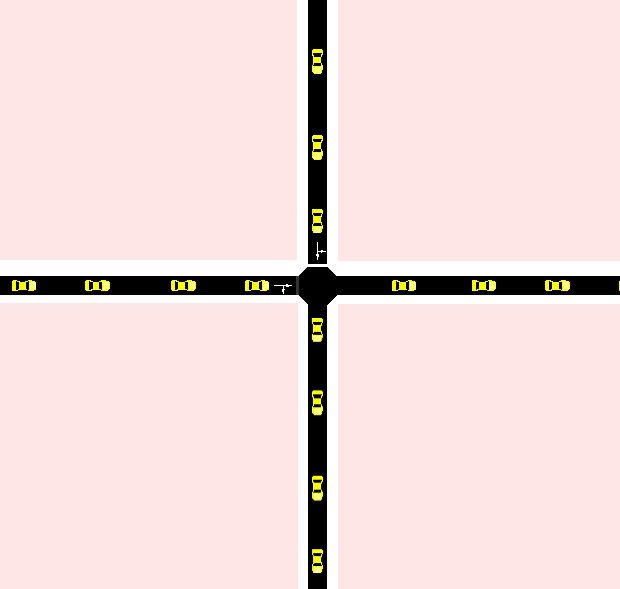
\includegraphics[width=.4\textwidth]{griglia-dettaglio-2.png}
% 	\end{center}
% 	\label{fig:griglia-dettaglio}\caption{Dettaglio della configurazione a griglia: in nero le strade e in giallo gli edifici.}
% \end{figure}
%
\subsection{Risultati}\label{sec:configurazione-griglia-risultati}
